\documentclass[12pt,letterpaper]{article}\usepackage[]{graphicx}\usepackage[]{color}
%% maxwidth is the original width if it is less than linewidth
%% otherwise use linewidth (to make sure the graphics do not exceed the margin)
\makeatletter
\def\maxwidth{ %
  \ifdim\Gin@nat@width>\linewidth
    \linewidth
  \else
    \Gin@nat@width
  \fi
}
\makeatother

\definecolor{fgcolor}{rgb}{0.345, 0.345, 0.345}
\newcommand{\hlnum}[1]{\textcolor[rgb]{0.686,0.059,0.569}{#1}}%
\newcommand{\hlstr}[1]{\textcolor[rgb]{0.192,0.494,0.8}{#1}}%
\newcommand{\hlcom}[1]{\textcolor[rgb]{0.678,0.584,0.686}{\textit{#1}}}%
\newcommand{\hlopt}[1]{\textcolor[rgb]{0,0,0}{#1}}%
\newcommand{\hlstd}[1]{\textcolor[rgb]{0.345,0.345,0.345}{#1}}%
\newcommand{\hlkwa}[1]{\textcolor[rgb]{0.161,0.373,0.58}{\textbf{#1}}}%
\newcommand{\hlkwb}[1]{\textcolor[rgb]{0.69,0.353,0.396}{#1}}%
\newcommand{\hlkwc}[1]{\textcolor[rgb]{0.333,0.667,0.333}{#1}}%
\newcommand{\hlkwd}[1]{\textcolor[rgb]{0.737,0.353,0.396}{\textbf{#1}}}%

\usepackage{framed}
\makeatletter
\newenvironment{kframe}{%
 \def\at@end@of@kframe{}%
 \ifinner\ifhmode%
  \def\at@end@of@kframe{\end{minipage}}%
  \begin{minipage}{\columnwidth}%
 \fi\fi%
 \def\FrameCommand##1{\hskip\@totalleftmargin \hskip-\fboxsep
 \colorbox{shadecolor}{##1}\hskip-\fboxsep
     % There is no \\@totalrightmargin, so:
     \hskip-\linewidth \hskip-\@totalleftmargin \hskip\columnwidth}%
 \MakeFramed {\advance\hsize-\width
   \@totalleftmargin\z@ \linewidth\hsize
   \@setminipage}}%
 {\par\unskip\endMakeFramed%
 \at@end@of@kframe}
\makeatother

\definecolor{shadecolor}{rgb}{.97, .97, .97}
\definecolor{messagecolor}{rgb}{0, 0, 0}
\definecolor{warningcolor}{rgb}{1, 0, 1}
\definecolor{errorcolor}{rgb}{1, 0, 0}
\newenvironment{knitrout}{}{} % an empty environment to be redefined in TeX

\usepackage{alltt}
 \usepackage[left=2cm,right=2cm,top=2cm,bottom=2cm]{geometry}
\usepackage[ansinew]{inputenc}
\usepackage[spanish]{babel}
\usepackage{amsmath}
\usepackage{amsfonts}
\usepackage{amssymb}
\usepackage{dsfont}
\usepackage{multicol} 
\usepackage{subfigure}
\usepackage{graphicx}
\usepackage{float} 
\usepackage{verbatim} 
\usepackage[left=2cm,right=2cm,top=2cm,bottom=2cm]{geometry}
\usepackage{fancyhdr}
\pagestyle{fancy} 
\fancyhead[LO]{\leftmark}
\usepackage{caption}
\newtheorem{definicion}{Definci\'on}
\IfFileExists{upquote.sty}{\usepackage{upquote}}{}
\begin{document}

\begin{titlepage}
\setlength{\unitlength}{1 cm} %Especificar unidad de trabajo


\begin{center}
\textbf{{\large UNIVERSIDAD DE EL SALVADOR}\\
{\large FACULTAD MULTIDISCIPLINARIA DE OCCIDENTE}\\
{\large DEPARTAMENTO DE MATEM\'ATICA}}\\[0.50 cm]

\begin{picture}(18,4)
 \put(7,0){
\includegraphics[width=4cm]{minerva.jpg}}
\end{picture}
\\[0.25 cm]

\textbf{{\large Licenciatura en Estad\'istica}\\[1.25cm]
{\large Control Estadistico del Paquete R }\\[2 cm]
%\setlength{\unitlength}{1 cm}
{\large  \textbf{''UNIDAD DOS"}}\\
{\large  \textbf{PR\'ACTICA 07 - AN\'ALISIS ESTAD\'ISTICO DE DATOS UNIVARIADOS DISCRETOS CON R.}}\\[3 cm]
{\large Alumna:}\\
{\large Martha Yoana Medina S\'anchez}\\[2cm]
{\large Fecha de elaboraci\'on}\\
Santa Ana - \today }
\end{center}
\end{titlepage}

\newtheorem{teorema}{Teorema}
\newtheorem{prop}{Proposici\'on}[section]

\lhead{UNIDAD DOS}
\chead{PRACTICA 07}
\lfoot{LICENCIATURA EN ESTAD\'ISTICA}
\cfoot{UESOCC}
\rfoot{\thepage}
%\pagestyle{fancy} 

\setcounter{page}{1}
\newpage

\begin{center}
\subsubsection*{\textbf{Pr\'actica 07-An\'alisis estad\'istico de datos univariados discretos con R.}}
\end{center}

\begin{center}
\subsection*{\textbf{AN\'ALISIS ESTAD\'ISTICO DE LOS DATOS.}}
\end{center}

\begin{enumerate}
  \item 

\begin{knitrout}
\definecolor{shadecolor}{rgb}{0.969, 0.969, 0.969}\color{fgcolor}\begin{kframe}
\begin{alltt}
\hlcom{# Activar el directorio de trabajo }

\hlkwd{getwd}\hlstd{()}
\end{alltt}
\begin{verbatim}
## [1] "C:/Users/User/Documents/PRACTICAS_YOANA_MEDINA/Yoana/PRACTICAS DE R"
\end{verbatim}
\begin{alltt}
\hlkwd{setwd}\hlstd{(}\hlstr{"C:/Users/User/Documents/PRACTICAS_YOANA_MEDINA/Yoana/PRACTICAS DE R"}\hlstd{)}
\end{alltt}
\end{kframe}
\end{knitrout}

\item 
\begin{knitrout}
\definecolor{shadecolor}{rgb}{0.969, 0.969, 0.969}\color{fgcolor}\begin{kframe}
\begin{alltt}
\hlcom{# Crear un nuevo Script y llamarle "Script07-DatosDiscretos"}
\end{alltt}
\end{kframe}
\end{knitrout}

\item 
\begin{knitrout}
\definecolor{shadecolor}{rgb}{0.969, 0.969, 0.969}\color{fgcolor}\begin{kframe}
\begin{alltt}
\hlcom{# Crear el vector de datos.}

\hlstd{Hijos} \hlkwb{<-} \hlkwd{c}\hlstd{(}\hlnum{2}\hlstd{,} \hlnum{1}\hlstd{)}
\hlkwd{data.entry}\hlstd{(Hijos)}
\hlstd{Hijos}
\end{alltt}
\begin{verbatim}
## [1] 2 1
\end{verbatim}
\begin{alltt}
\hlkwd{length}\hlstd{(Hijos)}
\end{alltt}
\begin{verbatim}
## [1] 2
\end{verbatim}
\end{kframe}
\end{knitrout}

\item
\begin{knitrout}
\definecolor{shadecolor}{rgb}{0.969, 0.969, 0.969}\color{fgcolor}\begin{kframe}
\begin{alltt}
\hlcom{# Guardar el vector de datos en un archivo de texto. }

\hlkwd{write}\hlstd{(Hijos,} \hlstr{"Hijos.txt"}\hlstd{)}
\end{alltt}
\end{kframe}
\end{knitrout}

\item
\begin{knitrout}
\definecolor{shadecolor}{rgb}{0.969, 0.969, 0.969}\color{fgcolor}\begin{kframe}
\begin{alltt}
\hlcom{# Limpiar el área de trabajo (Workspace)}

\hlkwd{ls}\hlstd{()}
\end{alltt}
\begin{verbatim}
## [1] "Hijos"
\end{verbatim}
\begin{alltt}
\hlkwd{rm}\hlstd{(}\hlkwc{list}\hlstd{=}\hlkwd{ls}\hlstd{(}\hlkwc{all}\hlstd{=}\hlnum{TRUE}\hlstd{));} \hlkwd{ls}\hlstd{()}
\end{alltt}
\begin{verbatim}
## character(0)
\end{verbatim}
\end{kframe}
\end{knitrout}

\item
\begin{knitrout}
\definecolor{shadecolor}{rgb}{0.969, 0.969, 0.969}\color{fgcolor}\begin{kframe}
\begin{alltt}
\hlcom{# Leer o recuperar el vector de datos o archivo de texto }

\hlstd{X} \hlkwb{<-} \hlkwd{scan}\hlstd{(}\hlstr{"Hijos.txt"}\hlstd{,} \hlkwc{what} \hlstd{=} \hlkwd{integer}\hlstd{(}\hlnum{0}\hlstd{),} \hlkwc{na.strings} \hlstd{=} \hlstr{"NA"}\hlstd{,} \hlkwc{flush}\hlstd{=}\hlnum{FALSE}\hlstd{)}
\hlkwd{ls}\hlstd{()}
\end{alltt}
\begin{verbatim}
## [1] "X"
\end{verbatim}
\end{kframe}
\end{knitrout}
\begin{knitrout}
\definecolor{shadecolor}{rgb}{0.969, 0.969, 0.969}\color{fgcolor}\begin{kframe}
\begin{alltt}
\hlcom{# Si el vector contiene caracteres se usa: }

\hlstd{what} \hlkwb{=} \hlkwd{character}\hlstd{()}
\end{alltt}
\end{kframe}
\end{knitrout}
\begin{knitrout}
\definecolor{shadecolor}{rgb}{0.969, 0.969, 0.969}\color{fgcolor}\begin{kframe}
\begin{alltt}
\hlcom{# Si el vector contiene reales se ocupa: }

 \hlstd{what} \hlkwb{=} \hlkwd{double}\hlstd{(}\hlnum{0}\hlstd{)}
\end{alltt}
\end{kframe}
\end{knitrout}

\item Elaborar el gr\'afico de puntos y diagrama de tallo-hojas (stem-and-leaf)

\begin{knitrout}
\definecolor{shadecolor}{rgb}{0.969, 0.969, 0.969}\color{fgcolor}\begin{kframe}
\begin{alltt}
\hlcom{# Grafico de puntos}

\hlkwd{stripchart}\hlstd{(X,} \hlkwc{method}\hlstd{=}\hlstr{"stack"}\hlstd{,} \hlkwc{vertical}\hlstd{=}\hlnum{FALSE}\hlstd{,} \hlkwc{col}\hlstd{=}\hlstr{"blue"}\hlstd{,} \hlkwc{pch}\hlstd{=}\hlnum{1}\hlstd{,}
\hlkwc{main}\hlstd{=}\hlstr{"Grafico de\textbackslash{}n puntos"}\hlstd{,} \hlkwc{xlab}\hlstd{=}\hlstr{"Numero de hijos"}\hlstd{)}
\end{alltt}
\end{kframe}
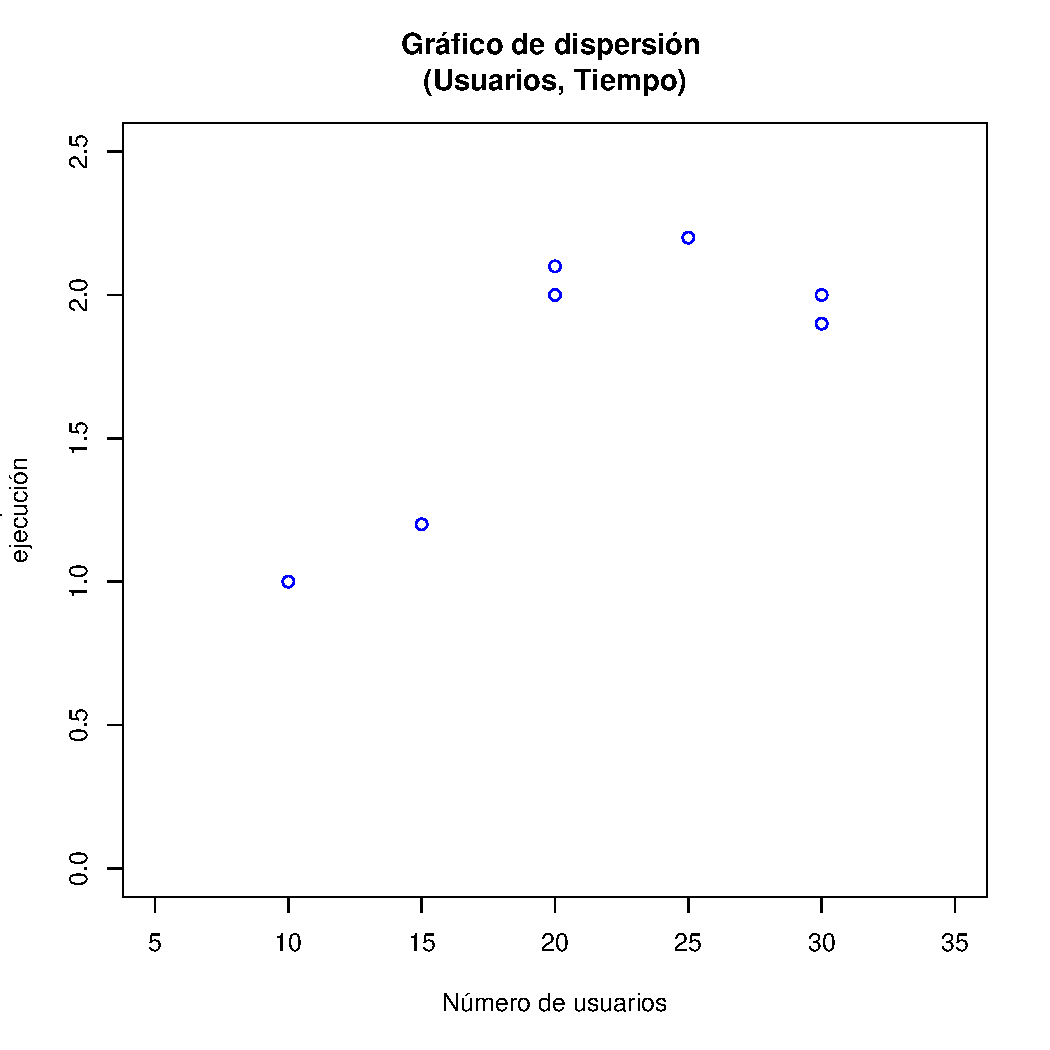
\includegraphics[width=\maxwidth]{figure/unnamed-chunk-9-1} 

\end{knitrout}

\textbf{Observaci\'on: method puede ser:} 

\textbf{"overplot" (los puntos coincidentes son superpuestos)}\\
\textbf{"jitter" (los puntos se ven como alejados o inquietos)}\\
\textbf{"stack" (los puntos coincidentes son apilados, uno tras otro)}\\

\begin{knitrout}
\definecolor{shadecolor}{rgb}{0.969, 0.969, 0.969}\color{fgcolor}\begin{kframe}
\begin{alltt}
\hlcom{# Gráfico de puntos}

\hlkwd{stripchart}\hlstd{(X,} \hlkwc{overplot}\hlstd{=}\hlstr{"stack"}\hlstd{,} \hlkwc{vertical}\hlstd{=}\hlnum{FALSE}\hlstd{,} \hlkwc{col}\hlstd{=}\hlstr{"blue"}\hlstd{,} \hlkwc{pch}\hlstd{=}\hlnum{1}\hlstd{,} \hlkwc{main}\hlstd{=}\hlstr{"Gráfico de\textbackslash{}n 
puntos"}\hlstd{,} \hlkwc{xlab}\hlstd{=}\hlstr{"Número de hijos"}\hlstd{)}
\end{alltt}


{\ttfamily\noindent\color{warningcolor}{\#\# Warning in plot.window(xlim, ylim, log, ...): "{}overplot"{} is not a graphical parameter}}

{\ttfamily\noindent\color{warningcolor}{\#\# Warning in axis(side = side, at = at, labels = labels, ...): "{}overplot"{} is not a graphical parameter}}

{\ttfamily\noindent\color{warningcolor}{\#\# Warning in title(xlab = xlab, ylab = ylab, ...): "{}overplot"{} is not a graphical parameter}}

{\ttfamily\noindent\color{warningcolor}{\#\# Warning in plot.xy(xy.coords(x, y), type = type, ...): "{}overplot"{} is not a graphical parameter}}\end{kframe}
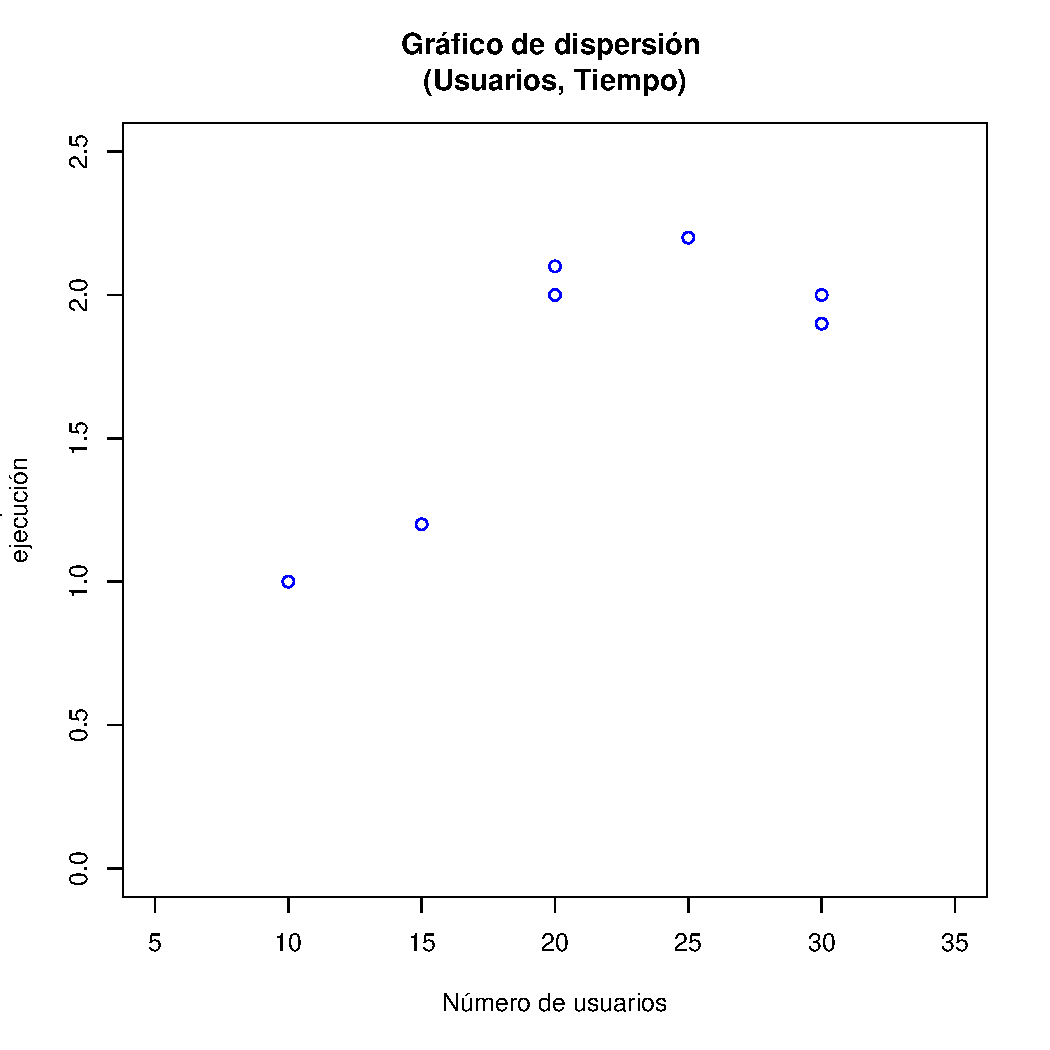
\includegraphics[width=\maxwidth]{figure/unnamed-chunk-10-1} 

\end{knitrout}
\begin{knitrout}
\definecolor{shadecolor}{rgb}{0.969, 0.969, 0.969}\color{fgcolor}\begin{kframe}
\begin{alltt}
\hlcom{# Gráfico de puntos }

\hlkwd{stripchart}\hlstd{(X,} \hlkwc{jitter}\hlstd{=}\hlstr{"stack"}\hlstd{,} \hlkwc{vertical}\hlstd{=}\hlnum{FALSE}\hlstd{,} \hlkwc{col}\hlstd{=}\hlstr{"blue"}\hlstd{,} \hlkwc{pch}\hlstd{=}\hlnum{1}\hlstd{,} \hlkwc{main}\hlstd{=}\hlstr{"Gráfico de\textbackslash{}n 
puntos"}\hlstd{,} \hlkwc{xlab}\hlstd{=}\hlstr{"Número de hijos"}\hlstd{)}
\end{alltt}
\end{kframe}
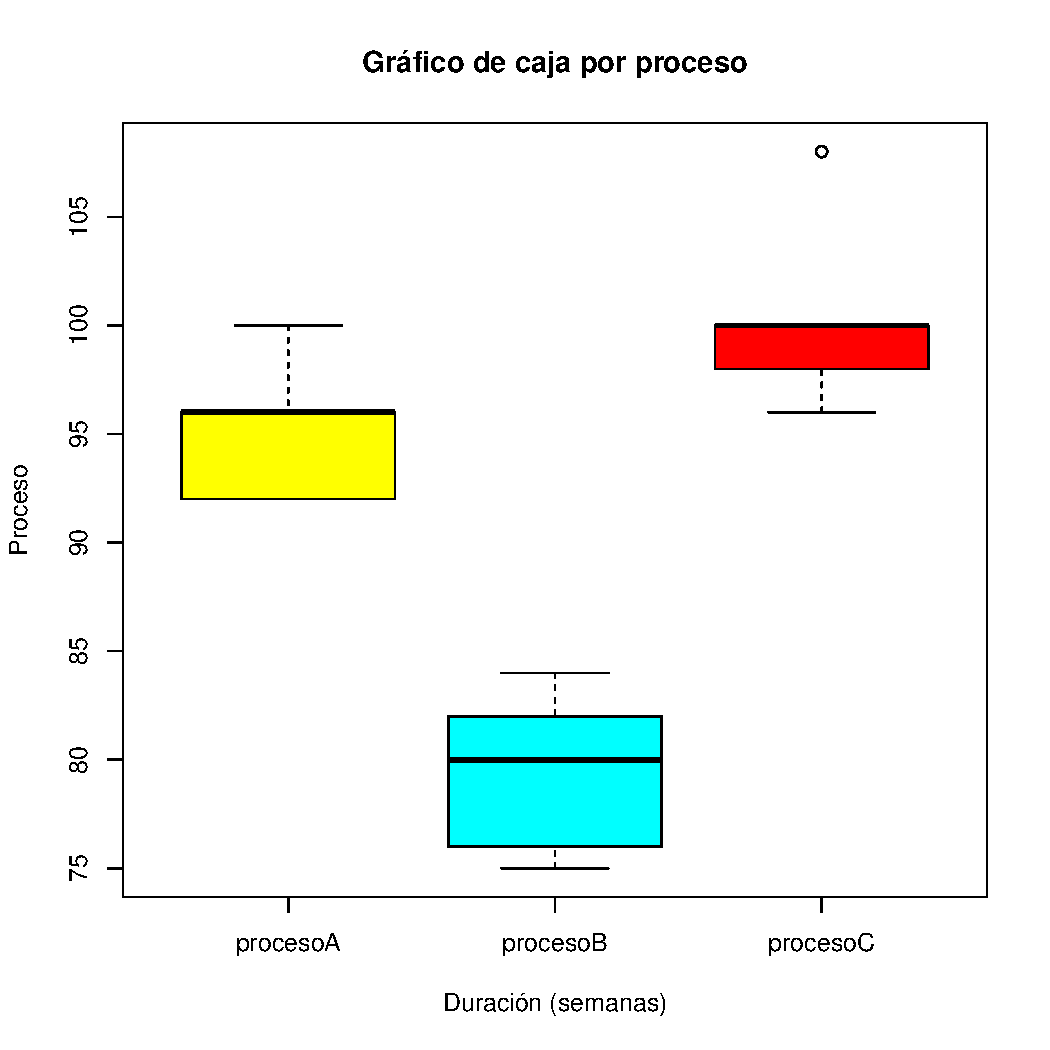
\includegraphics[width=\maxwidth]{figure/unnamed-chunk-11-1} 

\end{knitrout}
\begin{knitrout}
\definecolor{shadecolor}{rgb}{0.969, 0.969, 0.969}\color{fgcolor}\begin{kframe}
\begin{alltt}
\hlcom{# Gráfico de puntos }

\hlkwd{stripchart}\hlstd{(X,} \hlkwc{stack}\hlstd{=}\hlstr{"stack"}\hlstd{,} \hlkwc{vertical}\hlstd{=}\hlnum{FALSE}\hlstd{,} \hlkwc{col}\hlstd{=}\hlstr{"blue"}\hlstd{,} \hlkwc{pch}\hlstd{=}\hlnum{1}\hlstd{,} \hlkwc{main}\hlstd{=}\hlstr{"Gráfico de\textbackslash{}n 
puntos"}\hlstd{,} \hlkwc{xlab}\hlstd{=}\hlstr{"Número de hijos"}\hlstd{)}
\end{alltt}


{\ttfamily\noindent\color{warningcolor}{\#\# Warning in plot.window(xlim, ylim, log, ...): "{}stack"{} is not a graphical parameter}}

{\ttfamily\noindent\color{warningcolor}{\#\# Warning in axis(side = side, at = at, labels = labels, ...): "{}stack"{} is not a graphical parameter}}

{\ttfamily\noindent\color{warningcolor}{\#\# Warning in title(xlab = xlab, ylab = ylab, ...): "{}stack"{} is not a graphical parameter}}

{\ttfamily\noindent\color{warningcolor}{\#\# Warning in plot.xy(xy.coords(x, y), type = type, ...): "{}stack"{} is not a graphical parameter}}\end{kframe}
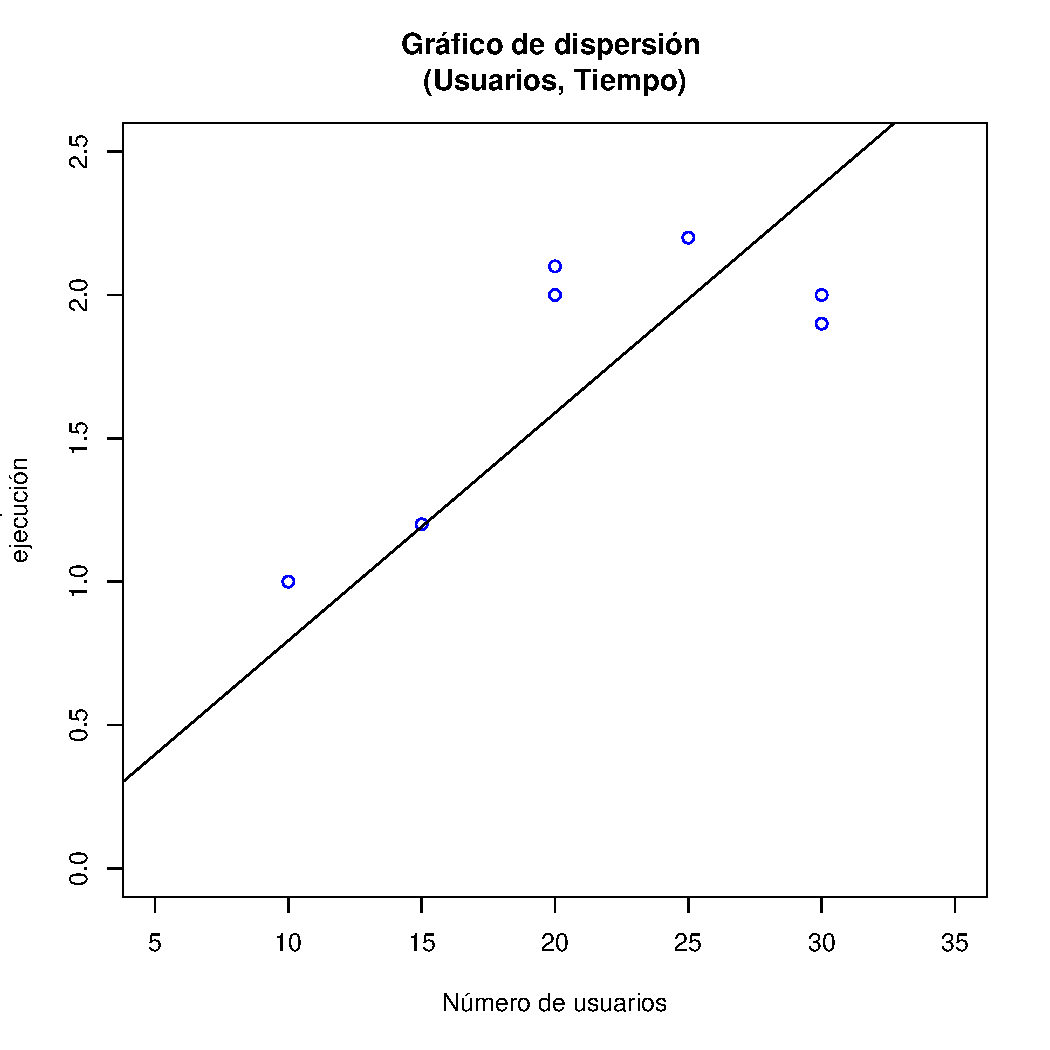
\includegraphics[width=\maxwidth]{figure/unnamed-chunk-12-1} 

\end{knitrout}

\item 
\begin{knitrout}
\definecolor{shadecolor}{rgb}{0.969, 0.969, 0.969}\color{fgcolor}\begin{kframe}
\begin{alltt}
\hlcom{# Crear la tabla de frecuencias completa }

\hlcom{# frecuencias individuales}

\hlstd{fab} \hlkwb{<-} \hlkwd{table}\hlstd{(X); fab} \hlcom{# frecuencias absolutas }
\end{alltt}
\begin{verbatim}
## X
## 1 2 
## 1 1
\end{verbatim}
\begin{alltt}
\hlstd{fre} \hlkwb{<-} \hlstd{fab}\hlopt{/}\hlkwd{length}\hlstd{(X); fre} \hlcom{# frecuencias relativas }
\end{alltt}
\begin{verbatim}
## X
##   1   2 
## 0.5 0.5
\end{verbatim}
\begin{alltt}
\hlstd{Fac} \hlkwb{<-} \hlkwd{cumsum}\hlstd{(fab); Fac} \hlcom{# frecuencias acumuladas }
\end{alltt}
\begin{verbatim}
## 1 2 
## 1 2
\end{verbatim}
\begin{alltt}
\hlstd{Far} \hlkwb{<-} \hlstd{Fac}\hlopt{/}\hlkwd{length}\hlstd{(X); Far} \hlcom{# frecuencias acumuladas relativas }
\end{alltt}
\begin{verbatim}
##   1   2 
## 0.5 1.0
\end{verbatim}
\end{kframe}
\end{knitrout}
\begin{knitrout}
\definecolor{shadecolor}{rgb}{0.969, 0.969, 0.969}\color{fgcolor}\begin{kframe}
\begin{alltt}
\hlcom{# tabla de frecuencias completa}

\hlkwd{options}\hlstd{(}\hlkwc{digits}\hlstd{=}\hlnum{2}\hlstd{)}
\hlstd{tabla} \hlkwb{<-} \hlkwd{data.frame}\hlstd{(}\hlkwc{fab}\hlstd{=fab,} \hlkwc{fre}\hlstd{=fre,} \hlkwc{Fac}\hlstd{=Fac,} \hlkwc{Far}\hlstd{=Far)}
\hlkwd{names}\hlstd{(tabla)} \hlkwb{<-} \hlkwd{c}\hlstd{(}\hlstr{"X"}\hlstd{,} \hlstr{"fab"}\hlstd{,} \hlstr{"free.X"}\hlstd{,} \hlstr{"fre"}\hlstd{,} \hlstr{"Fac"}\hlstd{,} \hlstr{"Far"}\hlstd{)}
\hlstd{tabla}
\end{alltt}
\begin{verbatim}
##   X fab free.X fre Fac Far
## 1 1   1      1 0.5   1 0.5
## 2 2   1      2 0.5   2 1.0
\end{verbatim}
\begin{alltt}
\hlstd{tfre} \hlkwb{<-} \hlkwd{data.frame}\hlstd{(}\hlkwc{X}\hlstd{=tabla}\hlopt{$}\hlstd{X,} \hlkwc{fab}\hlstd{=tabla}\hlopt{$}\hlstd{fab,} \hlkwc{fre}\hlstd{=tabla}\hlopt{$}\hlstd{fre,} \hlkwc{Fac}\hlstd{=tabla}\hlopt{$}\hlstd{Fac,}
                   \hlkwc{Far}\hlstd{=tabla}\hlopt{$}\hlstd{Far)}
\hlstd{tfre}
\end{alltt}
\begin{verbatim}
##   X fab fre Fac Far
## 1 1   1 0.5   1 0.5
## 2 2   1 0.5   2 1.0
\end{verbatim}
\end{kframe}
\end{knitrout}
\begin{knitrout}
\definecolor{shadecolor}{rgb}{0.969, 0.969, 0.969}\color{fgcolor}\begin{kframe}
\begin{alltt}
\hlcom{# Note que el cuadro resultante no tiene la presentacion deseada para }
\hlcom{# presentarla en un informe. Sin embargo, si estamos utilizando LATEX podemos }
\hlcom{# utilizar la siguiente instruccion xtable(tfre) y con esto nos genera el}
\hlcom{# codigo correspondiente para incorporarlo en nuestro archivo. }
\end{alltt}
\end{kframe}
\end{knitrout}

\item
\begin{knitrout}
\definecolor{shadecolor}{rgb}{0.969, 0.969, 0.969}\color{fgcolor}\begin{kframe}
\begin{alltt}
 \hlcom{# Calcular los estadisticos descriptivos de la variable}

\hlcom{# Estadisticos de tendencia central de los datos }

\hlstd{media} \hlkwb{<-} \hlkwd{mean}\hlstd{(X,} \hlkwc{na.rm} \hlstd{=} \hlnum{FALSE}\hlstd{); media}
\end{alltt}
\begin{verbatim}
## [1] 1.5
\end{verbatim}
\begin{alltt}
\hlcom{# na.rm = FALSE, le indica a R que los datos faltantes son omitidos en el  }
\hlcom{# calculo de la media. }
\end{alltt}
\end{kframe}
\end{knitrout}
\begin{knitrout}
\definecolor{shadecolor}{rgb}{0.969, 0.969, 0.969}\color{fgcolor}\begin{kframe}
\begin{alltt}
\hlkwa{for}\hlstd{(i} \hlkwa{in} \hlnum{1}\hlopt{:}\hlkwd{length}\hlstd{(X))} \hlkwa{if} \hlstd{(fab[i]} \hlopt{==} \hlkwd{max}\hlstd{(fab))} \hlkwa{break}\hlstd{()}
\hlstd{moda} \hlkwb{<-} \hlkwd{names}\hlstd{(fab[i]); moda}
\end{alltt}
\begin{verbatim}
## [1] "1"
\end{verbatim}
\begin{alltt}
\hlcom{# R no tiene incorporada una funcion para la moda}

\hlstd{mediana} \hlkwb{<-} \hlkwd{median}\hlstd{(X); mediana}
\end{alltt}
\begin{verbatim}
## [1] 1.5
\end{verbatim}
\end{kframe}
\end{knitrout}
\begin{knitrout}
\definecolor{shadecolor}{rgb}{0.969, 0.969, 0.969}\color{fgcolor}\begin{kframe}
\begin{alltt}
\hlcom{# Estadísticos de dispersión o variabilidad de los datos }

\hlkwd{range}\hlstd{(X)}
\end{alltt}
\begin{verbatim}
## [1] 1 2
\end{verbatim}
\begin{alltt}
\hlcom{# Devuelve el valor minimo y maximo del conjunto de datos. }
\end{alltt}
\end{kframe}
\end{knitrout}
\begin{knitrout}
\definecolor{shadecolor}{rgb}{0.969, 0.969, 0.969}\color{fgcolor}\begin{kframe}
\begin{alltt}
\hlstd{cuasivar} \hlkwb{<-} \hlkwd{var}\hlstd{(X); cuasivar}
\end{alltt}
\begin{verbatim}
## [1] 0.5
\end{verbatim}
\begin{alltt}
\hlstd{s} \hlkwb{<-} \hlkwd{sd}\hlstd{(X); s}
\end{alltt}
\begin{verbatim}
## [1] 0.71
\end{verbatim}
\begin{alltt}
\hlcom{# Devuelve la cuasivarianza y la cuasivarianza muestral }
\end{alltt}
\end{kframe}
\end{knitrout}
\begin{knitrout}
\definecolor{shadecolor}{rgb}{0.969, 0.969, 0.969}\color{fgcolor}\begin{kframe}
\begin{alltt}
\hlkwd{quantile}\hlstd{(X,}\hlkwd{c}\hlstd{(}\hlnum{0.25}\hlstd{,} \hlnum{0.5}\hlstd{,} \hlnum{0.75}\hlstd{))}
\end{alltt}
\begin{verbatim}
## 25% 50% 75% 
## 1.2 1.5 1.8
\end{verbatim}
\begin{alltt}
\hlcom{# Calculo de Q1, Q2, Q3 }
\end{alltt}
\end{kframe}
\end{knitrout}
\begin{knitrout}
\definecolor{shadecolor}{rgb}{0.969, 0.969, 0.969}\color{fgcolor}\begin{kframe}
\begin{alltt}
\hlkwd{quantile}\hlstd{(X,} \hlnum{0.6}\hlstd{)}
\end{alltt}
\begin{verbatim}
## 60% 
## 1.6
\end{verbatim}
\begin{alltt}
\hlcom{# En general se pueden encontrar cualquier percentil }
\end{alltt}
\end{kframe}
\end{knitrout}
\begin{knitrout}
\definecolor{shadecolor}{rgb}{0.969, 0.969, 0.969}\color{fgcolor}\begin{kframe}
\begin{alltt}
\hlcom{# Conocer un resumen de los datos }

\hlstd{resumen} \hlkwb{<-} \hlkwd{summary}\hlstd{(X); resumen}
\end{alltt}
\begin{verbatim}
##    Min. 1st Qu.  Median    Mean 3rd Qu.    Max. 
##     1.0     1.2     1.5     1.5     1.8     2.0
\end{verbatim}
\begin{alltt}
\hlcom{# Min, Q1, Median, Mean, Q3, Max }
\end{alltt}
\end{kframe}
\end{knitrout}
\begin{knitrout}
\definecolor{shadecolor}{rgb}{0.969, 0.969, 0.969}\color{fgcolor}\begin{kframe}
\begin{alltt}
\hlkwd{fivenum}\hlstd{(X)}
\end{alltt}
\begin{verbatim}
## [1] 1.0 1.0 1.5 2.0 2.0
\end{verbatim}
\begin{alltt}
\hlcom{# min, cuartil menor, mediana, cuartil mayor, max }
\end{alltt}
\end{kframe}
\end{knitrout}

\item Elaborar los gr\'aficos que se le pueden aplicar a la variable discreta

\begin{knitrout}
\definecolor{shadecolor}{rgb}{0.969, 0.969, 0.969}\color{fgcolor}\begin{kframe}
\begin{alltt}
\hlcom{# Grafico de barras (por ser pocos valores) }

\hlkwd{barplot}\hlstd{(tfre[[}\hlnum{2}\hlstd{]],} \hlkwc{main}\hlstd{=}\hlstr{"Gráfico de barras"}\hlstd{,} \hlkwc{xlab}\hlstd{=}\hlstr{"X = Número Hijos\textbackslash{}n"}\hlstd{,}
        \hlkwc{ylab}\hlstd{=}\hlstr{"frecuencia"}\hlstd{,} \hlkwc{col}\hlstd{=}\hlkwd{c}\hlstd{(}\hlstr{"yellow"}\hlstd{,} \hlstr{"blue"}\hlstd{,} \hlstr{"white"}\hlstd{,} \hlstr{"orange"}\hlstd{,}
                                 \hlstr{"cyan"}\hlstd{,} \hlstr{"red"}\hlstd{),} \hlkwc{sub}\hlstd{=}\hlstr{"Agosto-2012"}\hlstd{)}
\end{alltt}
\end{kframe}
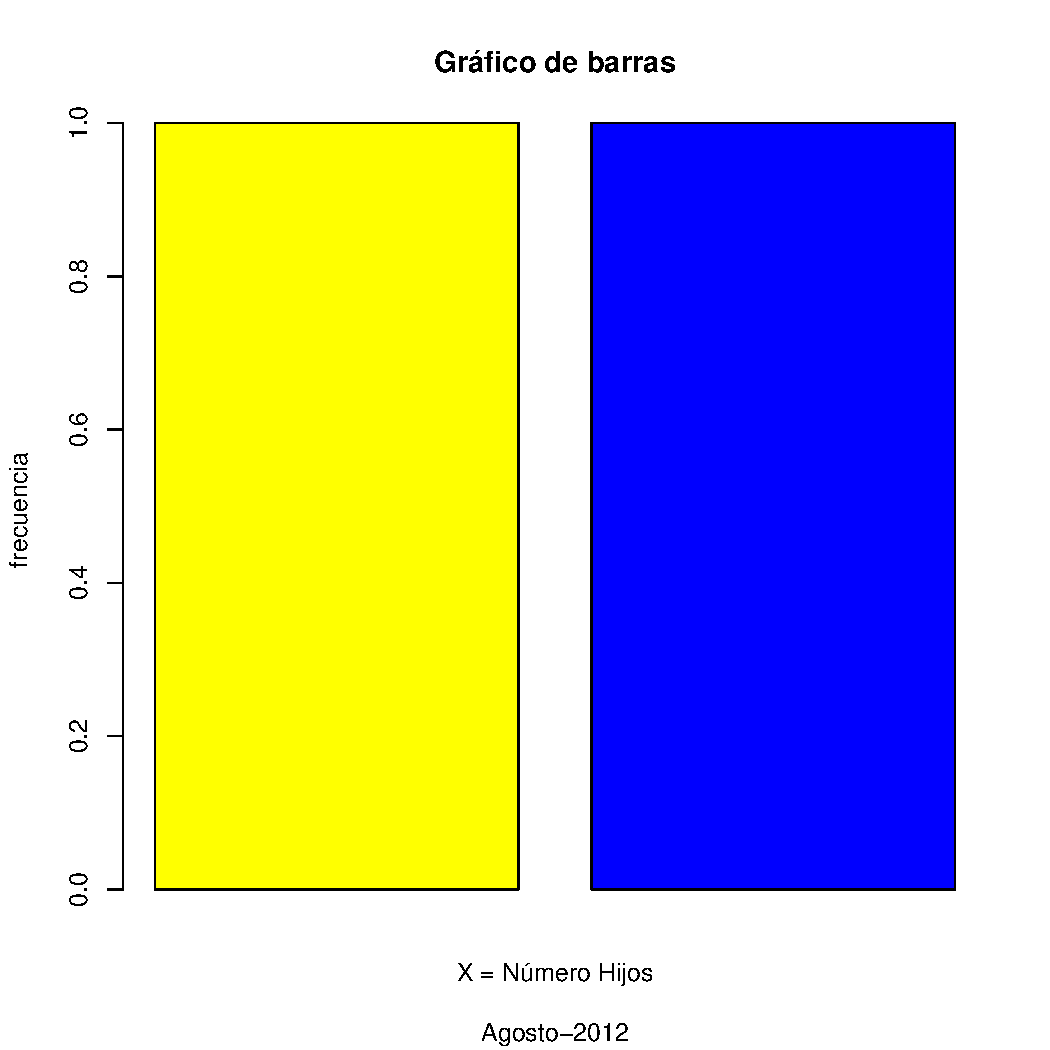
\includegraphics[width=\maxwidth]{figure/unnamed-chunk-24-1} 

\end{knitrout}

\begin{knitrout}
\definecolor{shadecolor}{rgb}{0.969, 0.969, 0.969}\color{fgcolor}\begin{kframe}
\begin{alltt}
\hlcom{# Grafico de pastel (por ser pocos valores)}

\hlkwd{pie}\hlstd{(tfre[[}\hlnum{2}\hlstd{]],} \hlkwc{main}\hlstd{=}\hlstr{"Gráfico de pastel"}\hlstd{,} \hlkwc{xlab}\hlstd{=}\hlstr{"Número Hijos \textbackslash{}n"}\hlstd{,}
    \hlkwc{col}\hlstd{=}\hlkwd{c}\hlstd{(}\hlstr{"orange"}\hlstd{,} \hlstr{"blue"}\hlstd{,} \hlstr{"white"}\hlstd{,} \hlstr{"yellow"}\hlstd{,} \hlstr{"cyan"}\hlstd{,} \hlstr{"blue"}\hlstd{),}
    \hlkwc{sub}\hlstd{=}\hlstr{"Agosto-2012"}\hlstd{)}
\end{alltt}
\end{kframe}
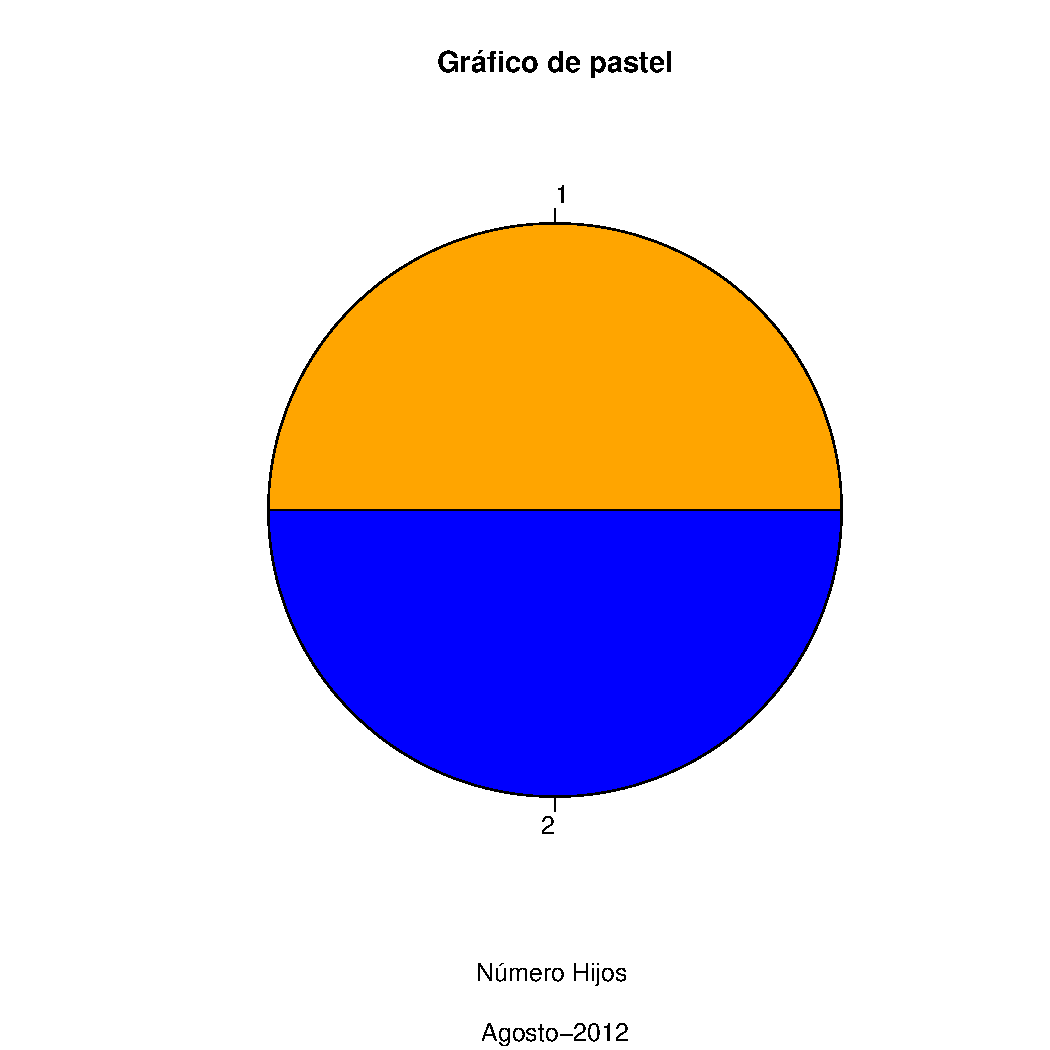
\includegraphics[width=\maxwidth]{figure/unnamed-chunk-25-1} 

\end{knitrout}

\begin{knitrout}
\definecolor{shadecolor}{rgb}{0.969, 0.969, 0.969}\color{fgcolor}\begin{kframe}
\begin{alltt}
\hlcom{# Se puede especificar nombres para las categorias }

\hlkwd{names}\hlstd{(fab)} \hlkwb{=} \hlkwd{c}\hlstd{(}\hlstr{"Cero"}\hlstd{,} \hlstr{"Uno"}\hlstd{)}

\hlkwd{pie}\hlstd{(fab,} \hlkwc{main}\hlstd{=}\hlstr{"Gráfico de pastel"}\hlstd{,} \hlkwc{xlab}\hlstd{=}\hlstr{"X = Número Hijos\textbackslash{}n"}\hlstd{,}
    \hlkwc{col}\hlstd{=}\hlkwd{c}\hlstd{(}\hlstr{"yellow"}\hlstd{,} \hlstr{"blue"}\hlstd{,} \hlstr{"white"}\hlstd{,} \hlstr{"orange"}\hlstd{,} \hlstr{"cyan"}\hlstd{,} \hlstr{"red"}\hlstd{),}
    \hlkwc{sub}\hlstd{=}\hlstr{"Agosto-2012"}\hlstd{)}
\end{alltt}
\end{kframe}
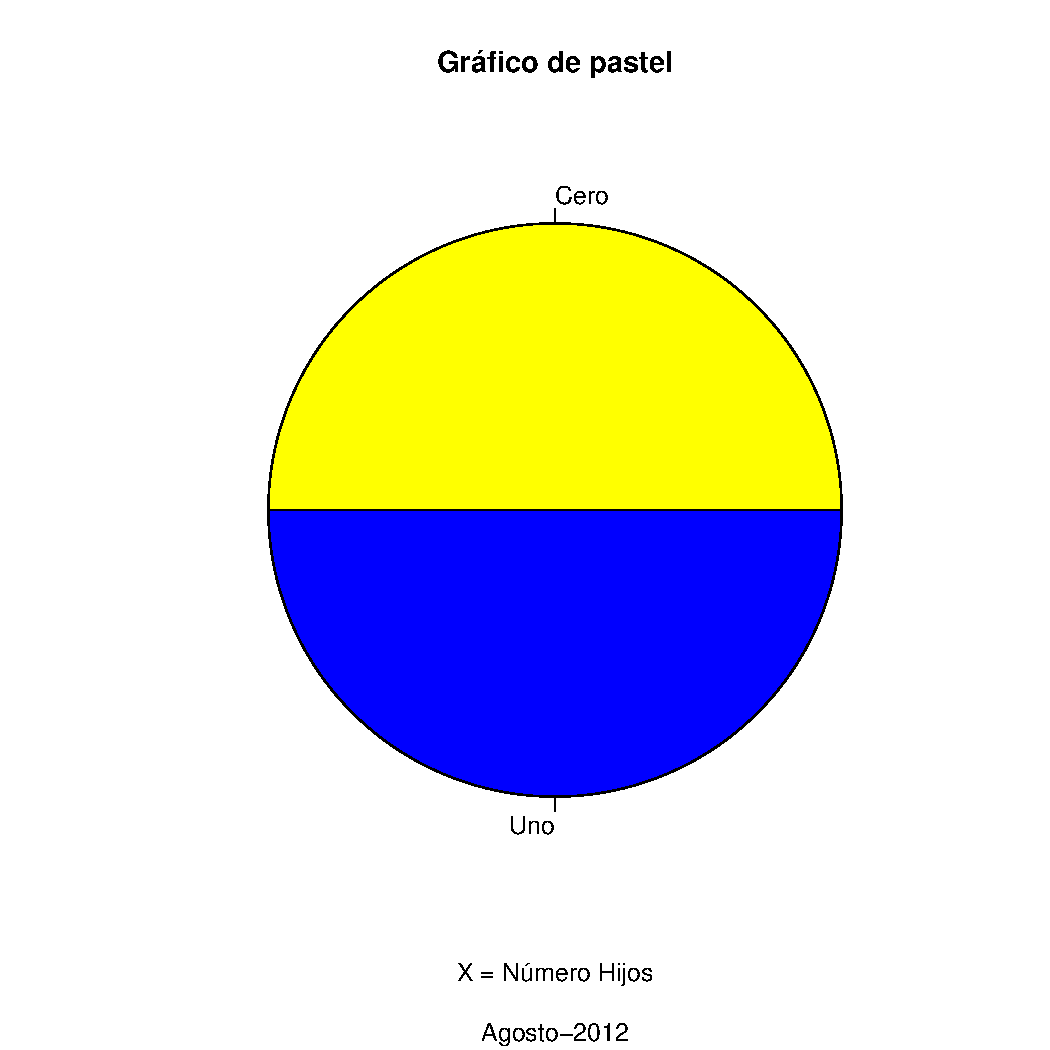
\includegraphics[width=\maxwidth]{figure/unnamed-chunk-26-1} 

\end{knitrout}

\begin{knitrout}
\definecolor{shadecolor}{rgb}{0.969, 0.969, 0.969}\color{fgcolor}\begin{kframe}
\begin{alltt}
\hlcom{# Gráfico de cajas (box-plot) es la representación gráfica de los cinco }
\hlcom{# numeros Horizontal}

\hlkwd{boxplot}\hlstd{(X,} \hlkwc{main}\hlstd{=}\hlstr{"Gráfico de caja"}\hlstd{,} \hlkwc{ylab}\hlstd{=}\hlstr{"Número de hijos\textbackslash{}n"}\hlstd{)}
\end{alltt}
\end{kframe}
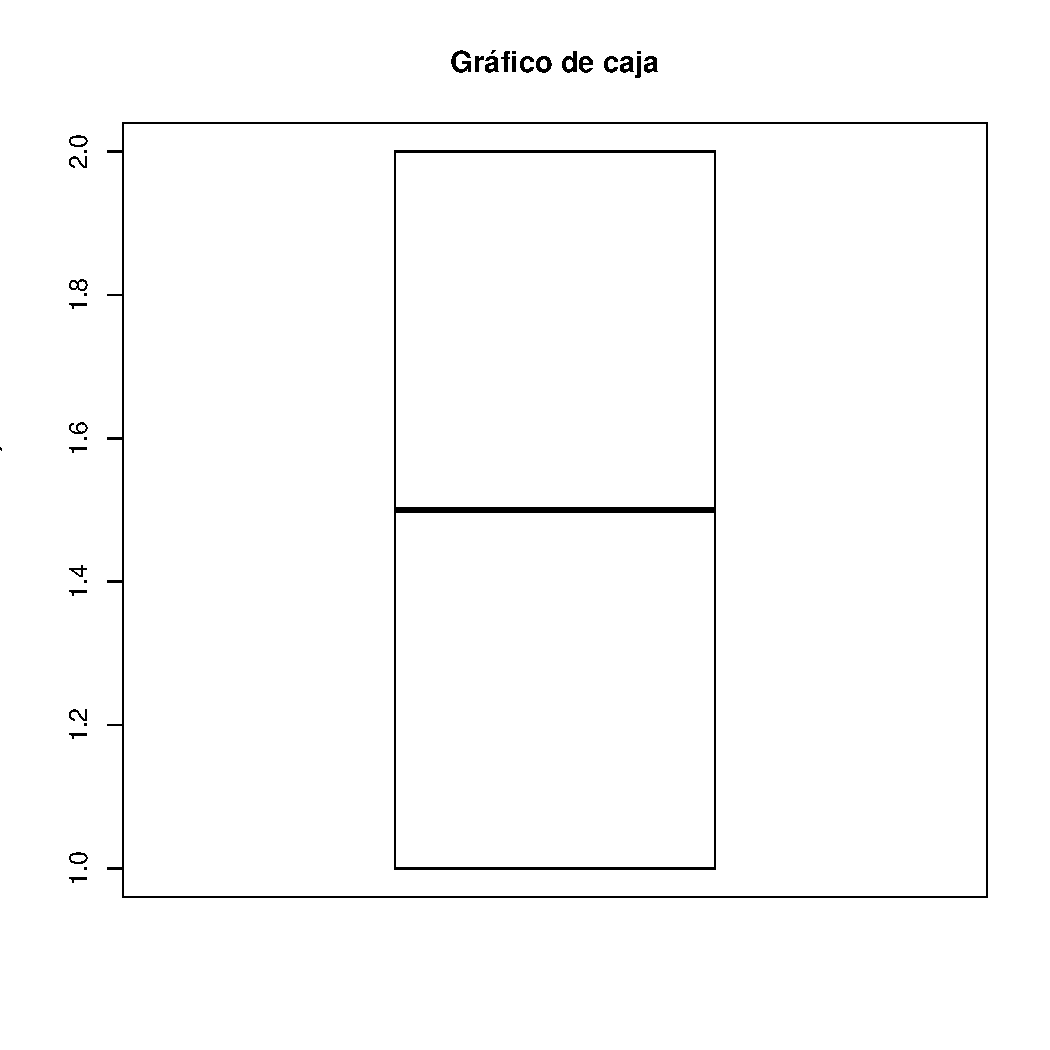
\includegraphics[width=\maxwidth]{figure/unnamed-chunk-27-1} 

\end{knitrout}

\begin{knitrout}
\definecolor{shadecolor}{rgb}{0.969, 0.969, 0.969}\color{fgcolor}\begin{kframe}
\begin{alltt}
\hlcom{# Vertical }

\hlkwd{boxplot}\hlstd{(X,} \hlkwc{main}\hlstd{=}\hlstr{"Gráfico de caja"}\hlstd{,} \hlkwc{xlab}\hlstd{=}\hlstr{" Número de hijos\textbackslash{}n"}\hlstd{,} \hlkwc{plot}\hlstd{=}\hlnum{TRUE}\hlstd{,}
        \hlkwc{border}\hlstd{=}\hlstr{"red"}\hlstd{,} \hlkwc{col}\hlstd{=}\hlstr{"yellow"}\hlstd{,} \hlkwc{horizontal}\hlstd{=}\hlnum{TRUE}\hlstd{)}
\end{alltt}
\end{kframe}
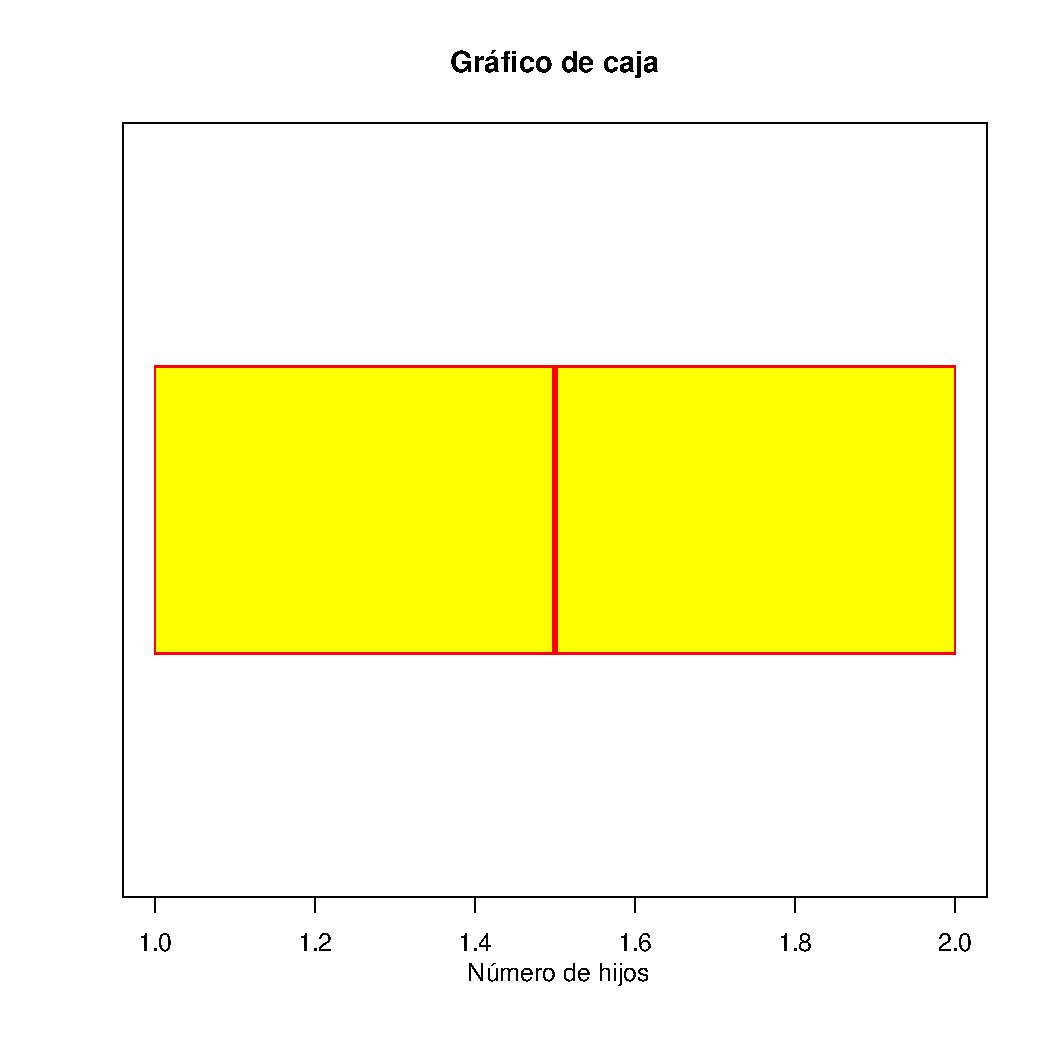
\includegraphics[width=\maxwidth]{figure/unnamed-chunk-28-1} 

\end{knitrout}

\begin{knitrout}
\definecolor{shadecolor}{rgb}{0.969, 0.969, 0.969}\color{fgcolor}\begin{kframe}
\begin{alltt}
\hlcom{# NOTE QUE TODOS LOS GRAFICOS DE BARRAS Y DE PASTEL SON REALIZADOS }
\hlcom{# APARTIR DE UNA TABLA DE FRECUENCIA, LA CUAL SE INDICA EN tfre[[2]]. }
\hlcom{# TAMBIEN SE PUDO UTILIZAR tabla[[2]]. }
\end{alltt}
\end{kframe}
\end{knitrout}
























\end{enumerate}




\end{document}
